\documentclass[a4paper,12pt]{report}

\title{Embedding intuitionistic into classical logic}
\author{Alexander Pluska}

\usepackage{amsmath,amssymb,amsthm}
\usepackage{ wasysym }
\usepackage{ stmaryrd }
\usepackage{ mathpartir }
\usepackage{bussproofs}
\usepackage{enumerate}
\usepackage{tikz-qtree}
\usetikzlibrary{positioning}
\usetikzlibrary{arrows.meta}
\usepackage{stackengine}
\usepackage{bbold}
\usepackage{footmisc}


\usepackage{hyperref}% http://ctan.org/pkg/hyperref
\usepackage{cleveref}% http://ctan.org/pkg/cleveref

\theoremstyle{definition}
\newtheorem{theorem}{Theorem}[section]
\theoremstyle{definition}
\newtheorem{corollary}[theorem]{Corollary}
\theoremstyle{definition}
\newtheorem{lemma}[theorem]{Lemma}
\theoremstyle{definition}
\newtheorem{proposition}[theorem]{Proposition}
\theoremstyle{definition}
\newtheorem{definition}[theorem]{Definition}
\theoremstyle{definition}
\newtheorem{example}[theorem]{Example}
\theoremstyle{definition}
\newtheorem{remark}[theorem]{Remark}

\DeclareMathOperator*{\argmax}{arg\,max}

\begin{document}
	
	\maketitle
	
	\begin{abstract}
		We present an embedding of intuitionistic into classical logic, a quasi-inverse to the famous double-negation translation, i.e. a procedure that for each formula $\varphi$ gives a formula $\varphi_c$ such that $\varphi$ is intuitionistically valid if and only if $\varphi_c$ is classically valid. We consider both the propositional and predicate case. Since many of the more involved results for the more interesting predicate scenario involve similar arguments as in the propositional case we shall develop them simultaneously.
	\end{abstract}
	
	\tableofcontents

	\chapter{Preliminaries}

	First let us recapitulate the most important definitions and some facts about them. This will serve to fix our notation as well.
	
	\section{Syntax}
	
	\subsection{Propositional logic}
	
	Let us fix some countably infinite set of propositional variables $A, B, C\dots$.
	
	\begin{definition}
		A \textit{formula} and \textit{subformula} is defined inductively via the following rules:
		\begin{itemize}
			\item every propositional variable as well as a special symbol $\bot$ is a formula, such a formula is called \textit{atomic} and $A,B,C,\dots$ and $\bot$ are called \textit{atoms}.
			\item if $\varphi$ and $\psi$ are formulas then $\varphi\circ\psi$ is a formula for $\circ\in\{\wedge,\vee,\to\}$.
			\item every formula is a subformula of itself.
			\item for a formula $\chi = \varphi\circ\psi$ every subformula of $\varphi$ and $\psi$ is also a subformula of $\chi$.
		\end{itemize}
	We write $\neg \varphi$ for $\varphi\to \bot$.
	\end{definition}

	\subsection{Predicate logic}
	
	The analog for predicate logic is much more involved as we need to define the term language.
	
	\begin{definition}
		A \textit{signature} consists of
		\begin{itemize}
			\item a finite set $S_f$ of function symbols $f_1, \dots, f_n$
			\item a finite set $S_R$ of relation symbols $R_1,\dots, R_m$
			\item  a function ar$: S_f\cup S_R\to \mathbb{N}$ assigning to each symbol its arity (possibly 0).
		\end{itemize}
	\end{definition}
	
	\noindent Usually the signature we be left implicit. If explicitly stated we denote it by $$\{f_1/\text{ar}(f_1),\dots,f_n/\text{ar}(f_n), R_1/\text{ar}(R_1).\dots,R_m/\text{ar}(R_m)\}.$$
	Fix a countably infinite collection of free variables $a, b, c\dots$ and bound variables $x, y, z\dots$.
	Note that the following definitions could be simplified by not distinguishing between bound and free variables. However this has some other drawbacks and in particular when defining a sequent calculus for first-order logic having disjoint sets of bound and free variables is convenient.
	
	\begin{definition}
		A \textit{term} is defined inductively via the following rules
		\begin{itemize}
			\item each free variable is a term
			\item if $t_1,\dots,t_n$ are terms and $f$ an $n$-ary function symbol then $f(t_1, \dots, t_n)$ is a term.
		\end{itemize}
		A \textit{semiterm} is defined in the same way with the difference that bound variables are allowed in 1. Clearly every term is a semiterm. Analogously to before we can define \textit{subterms} and \textit{subsemiterms}.
	\end{definition}

	\begin{definition}
		A \textit{Substitution} is a function $\sigma$ from free variables to semiterms. For a semiterm $t$ we define $t\sigma$ as follows:
		\begin{itemize}
			\item $x\sigma = x$ if $x$ is bound.
			\item $a\sigma = \sigma(a)$ if $a$ is free.
			\item $f(t_1,\dots,t_n)\sigma = f(t_1\sigma,\dots,t_n\sigma)$.
		\end{itemize}
	\end{definition}
	
	\begin{definition}
		A \textit{formula} is defined inductively via the following rules
		\begin{itemize}
			\item $\bot$ is a formula.
			\item if $t_1,\dots,t_n$ are terms and $R$ and an $n$-ary relation symbol then $R(t_1, \dots, t_n)$ is a formula.
			\item if $s, t$ are terms then $s = t$ is a formula.
		\end{itemize}	
		Formulas formed by the above rules are called \textit{atomic}.
		\begin{itemize}
			\item If $\varphi$ and $\psi$ are formulas then $\varphi\circ\psi$ is a formula for $\circ\in\{\wedge,\vee,\to\}$.
			\item If $\varphi$ is a formula and $a$ is a free variable occurring in $\varphi$ and $x$ is a bound variable not occurring in $\varphi$ then $Qx(\varphi[x/a])$ is a formula for $Q\in\{\exists,\forall\}$ where the \textit{substitution} $\varphi\sigma$ is defined inductively via
			\begin{itemize}
				\item $\bot\sigma = \bot$
				\item $R(t_1,\dots,t_n)\sigma = R(t_1\sigma,\dots, t_n\sigma)$
				\item $(s = t)\sigma = (s\sigma = t\sigma)$
				\item $(\varphi\circ\psi)\sigma = \varphi\sigma\circ\psi\sigma$ for $\circ\in\{\wedge,\vee,\to\}$.
				\item $(Qy\varphi)\sigma = Qy(\varphi\sigma)$ for $Q\in\{\exists,\forall\}$.
			\end{itemize}
			\item A formula with no free variables is a \textit{sentence}.
		\end{itemize}
	\end{definition}

	\section{Semantics}
	
	We now give meaning to formulas in classical and intuitionistic logic.
	
	\subsection{Propositional Logic}
	\subsubsection{Classical Semantics}
	
	\begin{definition}
		A \textit{valuation} $v$ is a function that assigns to each propositional variable $A$ a \textit{true value} $v(A)\in\{0, 1\}$. We extend $v$ to a function $v^*$ on formulas:
		\begin{itemize}
			\item $v^*(\bot) = 0$
			\item $v^*(A) = v(A)$ for each propositional variable $A$.
			\item $v^*(\varphi\wedge\psi) = \min(v^*(\varphi), v^*(\psi))$
			\item $v^*(\varphi\vee\psi) = \max(v^*(\varphi), v^*(\psi))$
			\item $v^*(\varphi\to \psi) = \max(1 - v^*(\varphi), v^*(\psi))$
		\end{itemize}
		$v$ is a \textit{model} for $\varphi$ if $v(\varphi) = 1$, we write $v\models\varphi$. $\varphi$ is \textit{satisfiable} if there exists a valuation which is a model. It is \textit{valid} if every valuation is a model and we write $\models \varphi$. We denote the set of valid formulas with CPC. We can furthermore define an entailment relation between sets of clauses, that is $\mathcal S\models_C \mathcal T$ if for every valuation $v$ with $v\models\bigwedge S$ we have $v\models\bigvee \mathcal T$.
	\end{definition}
	
	One notable property of classical logic is that a formula $\varphi$ is valid if and only if its negation, i.e. $\neg\varphi$ is not satisfiable. The same does not hold true for intuitionistic logic as we shall see.

	\subsubsection{Intuitionistic Semantics}
	
	\begin{definition}
		A \textit{Kripke structure} $\mathcal K = (W, (v_w)_{w\in W})$ consists of a partially ordered set $W$ of nodes an a family of valuations $(v_w)_{w\in W}$ such that for $u\leq w$ we have $v_u(A)\leq v_u(A)$ for every propositional variable $A$, this is called the \textit{persistency condition}. We extend the valuations $v_u$ slightly differently to $v_u^\#$ than before, i.e. have
		\begin{itemize}
			\item $v_u^\#(\bot) = 0$
			\item $v_u^\#(\varphi) = v_u(A)$ if $\varphi$ is atomic.
			\item $v_u^\#(\varphi\wedge\psi) = \min(v_u^\#(\varphi), v_u^\#(\psi))$
			\item $v_u^\#(\varphi\vee\psi) = \max(v_u^\#(\varphi), v_u^\#(\psi))$
			\item $v_u^\#(\varphi\to \psi) = \min\{\max(1 - v_w^\#(\varphi), v_w^\#(\psi))\:|\:w\geq u\}$
		\end{itemize}
		That is $v_u^\#(\varphi\to \psi) = 1$ if at every world $w\geq u$ we have $v_w^\#(\varphi) = 0$ or $v_w^\#(\psi) = 1$. We say that $\varphi$ is satisfied at a node $u$ if $v_u^\#(\varphi) = 1$ and write $u\models\varphi$. If a formula is satisfied at every node $K$ is a \textit{model} for $\varphi$ and we write $K\models \varphi$. $\varphi$ is satisfiable if there exists a Kripke structure which is a model. It is \textit{valid} if every Kripke structure is a model and we write $\models \varphi$. We denote the set of valid formulas with IPC. As before we define an entailment relation $\models_I$ between sets of formulas.
	\end{definition}
	There are many classical tautologies which are not intuitionistically valid
	\begin{example}\label{LEMcounterexample}
		Consider the famous law of excluded middle $A\vee\neg A$. As a counter model consider a Kripke structure with two nodes $u\leq w$ and $v_u(A) = 0, v_w(A) = 1$. Then $u\not\models A$ and $u\not\models \neg A$, i.e. $u\not\models A\vee\neg A$. 
	\end{example}
	The following is a famous and important result due to Glivenko~\cite{glivenko1929}
	
	\begin{theorem}[Glivenko's theorem]
		A propositional formula $\varphi$ is classically valid if and only if $\neg\neg\varphi$ is intuitionistically valid.
	\end{theorem}
	\noindent Note however that this difference between classical and intuitionistic logic is not reflected in satisfiability, only in validity:
	\begin{lemma}\label{propsat}
		A propositional formula $\varphi$ is intuitionistically satisfiable if and only if it is classically satisfiable.
	\end{lemma}

	\begin{proof}
		Every classical model can be viewed as a Kripke model with a single node. Therefore classical satisfiability trivially implies intuitionistic satisfiability.	On the other hand in every Kripke structure that is a model every node is a classical model so intuitionistic satisfiability implies intuitionistic satisfiability.
	\end{proof}

	In classical logic a proven strategy for showing that a formula valid is to consider its negation and show that it is not satisfiable. Due to the previous lemma this is insufficient for intuitionistic logic. There are formulas like $A\vee\neg A$ which are not a intuitionistic tautology while their negation is not satisfiable either. This serves to motivate the consideration of equivalidity in the following chapters. In the context of classical logic it can be fully explained via equisatisfiability and is therefore neglected but for intuitionistic logic it is more fundamental.
	
	Finally let us note the complexities of these various decision problems, which play a fundamental role in all of theoretical computer science.
	
	\begin{theorem}
		Satisfiability for classical and intuitionistic propositional logic is NP-complete.
	\end{theorem}

	For classical logic this is the famous Cook-levin theorem first published in Cook's seminal paper~\cite{cook1971complexity}. Of course we have seen that the intuitionistic case is the same decision problem.
	
	\begin{corollary}
		Validity for classical logic is co-NP-complete
	\end{corollary}

	This is clear since validity is just the complementary problem to satisfiability of the negated formula. However in intuitionistic logic unfortunately validity is really harder than satisfiability as shown by Statman~\cite{statman1979intuitionistic}.
	
	\begin{theorem}
		Validity for intuitionistic logic in PSPACE-complete.
	\end{theorem}

	One thing to note is that in contrast to predicate logic all these problems are decidable.
	
	
	\subsection{Predicate Logic}

	We now give account of the more involved semantics of first-order logic
	
	\subsubsection{Classical Semantics}

	\begin{definition}
		Let $\Sigma$ be a signature. A $\Sigma$-structure $\mathcal{M}$ consists of a non-empty set $M$, the domain of $\mathcal{M}$, and a function $I$ that assigns
		\begin{itemize}
			\item to each $n$-ary function symbol $f$ a $n$-ary function $f^I: M^n\to M$.\footnote{Here $f|_M$ denotes the restriction of $f$ to $M$}
			\item to each $n$-ary relation symbol $R$ a $n$-ary relation $R^I\subseteq M^n$.
		\end{itemize}
		A variable assignment $v$ is a function that assigns to each free variable an element $m\in M$. For each free variable $a$ and $m\in M$ we define $$v[m/a](b) = \begin{cases}
			m&\text{if $b=a$}\\
			v(b)&\text{otherwise}
		\end{cases}$$
		Then terms are interpreted as follows:
		\begin{itemize}
			\item $a^{I, v} = v(a)$ for each free variable $a$.
			\item $f(t_1,\dots,t_n)^{I, v} = f^I(t_1^{I, v},\dots, t_n^{I, v})$.
		\end{itemize}
		We define a model relation between pairs $\mathcal M, v$ and formulas $\varphi$ as follows
		\begin{itemize}
			\item $\mathcal M, v\not\models\bot$.
			\item $\mathcal M, v\models R(t_1,\dots,t_n)$ iff $(t_1^{I, v},\dots,t_n^{I, v})\in R^I$.
			\item $\mathcal M, v\models s = t$ iff $s^{I, v} = t^{I, v}$.
			\item $\mathcal M, v\models \varphi\wedge \psi$ iff $\mathcal M, v\models\varphi$ and $\mathcal M, v\models\psi$.
			\item $\mathcal M, v\models \varphi\vee\psi$ iff $\mathcal M, v\models\varphi$ or $\mathcal M, v\models\psi$.
			\item $\mathcal M, v\models \varphi\to\psi$ iff $\mathcal M, v\not\models\varphi$ or $\mathcal M, v\models\psi$.
			\item $\mathcal M, v\models\exists x\varphi$ iff there exists $m\in M$ such that $\mathcal M, v[m/a]\models\varphi[a/x]$ where a is a free variable that does not occur in $\varphi$.
			\item $\mathcal M, v\models\forall x\varphi$ iff for all $m\in M$ we have $\mathcal M, v[m/a]\models\varphi[a/x]$ where a is a free variable that does not occur in $\varphi$.
		\end{itemize}
		$\varphi$ is satisfiable if for some $\mathcal{M}, v$ we have  $\mathcal M, v\models\varphi$. It is valid if for all  $\mathcal M, v$ we have  $\mathcal M, v\models\varphi$. We write $\mathcal{M}\models\varphi$ if for every $v$ we have  $\mathcal M, v\models\varphi$. We denote the set of valid formulas with CQC. As before define an entailment relation $\models_C$ between sets of formulas.
	\end{definition}

	\subsubsection{Intuitionistic Semantics}
	
	\begin{definition}
		A $\Sigma$-\textit{Kripke structure} $\mathcal{K}$ is a partially ordered set $W$ and a family of $\Sigma$-structures $(\mathcal{M}_w)_{w\in W}$ such that for $u\leq w$
		\begin{itemize}
			\item $M_u\subseteq M_w$.
			\item $f^{I_w}|_{M_u} = f^{I_u}$.
			\item $R^{I_w}|_{M_u} = f^{I_u}$.
		\end{itemize}
		Then we define a model relation between worlds $u\in W$ and variable assignments $v$ (targeting $M_u$) and formulas $\varphi$ as follows:
		\begin{itemize}
			\item $u, v\not\models\bot$
			\item $u, v\models R(t_1,\dots,t_n)$ iff $(t_1^{I_u, v},\dots,t_n^{I_u, v})\in R^{I_u}$.
			\item $u, v\models s = t$ iff $s^{I_u, v} = t^{I_u, v}$.
			\item $u, v\models \varphi\wedge \psi$ iff $u, v\models\varphi$ and $u, v\models\psi$.
			\item $u, v\models \varphi\vee\psi$ iff $u, v\models\varphi$ or $u, v\models\psi$.
			\item $u, v\models \varphi\to\psi$ iff for every $w\geq u$ we have $w, v\not\models\varphi$ or $w, v\models\psi$.
			\item $u, v\models\exists x\varphi$ iff there exists $m\in M_u$ such that $u, v[m/a]\models\varphi[a/x]$ where a is a free variable that does not occur in $\varphi$.
			\item $u, v\models\forall x\varphi$ iff for every $w\geq u$ and $m\in M_w$ we have $w, v[m/a]\models\varphi[a/x]$ where a is a free variable that does not occur in $\varphi$.
		\end{itemize}
		We say that $\mathcal{K}$ satisfies $\varphi$ if $u, v\models\varphi$ holds for every world $u$ and variable assignment $v$. As always a formula is satisfiable if it is satisfies by some Kripke structure and it is valid if it is satisfied in every Kripke structure. We denote the set of valid formulas with IQC.  As before define an entailment relation $\models_I$ between sets of formulas.
	\end{definition}
	In addition to the propositional tautologies there are now sentences involving quantifiers which are classically valid but not intuitionistically.
	Consider for instance the classical tautology $\varphi$ $$\neg\forall x A(x)\to \exists x \neg A(x)$$We exhibit an intuitionistic counter model. Consider the Kripke structure with two nodes $u\leq w$ with $M_u = \{0\}, M_w = \{0, 1\}$ and $A^{I_u} = A^{I_w} = \{0\}$. Then $u, v\not\models \varphi$: First note that $w, v\not\models\forall xA(x)$ and $u, v\not\models\forall xA(x)$ for any valuation $v$ since $w, v[1, a]\not\models A(a)$, i.e. $u, v\models\neg\forall xA(x)$ and also $w, v\models\neg\forall xA(x)$. Furthermore $u, v[0/a]\not\models \neg A(a)$ and $w, v[0/a]\not\models \neg A(a)$ so $u, v\not\models \exists x\neg A(x)$ for any valuation $v$ (note however that this is not true at $w$!). Therefore $u, v\not\models\varphi$.
	
	Intuitively the problem is that the existential quantifier at $u$ does not see the elements at $w$, i.e. it must "choose" between the currently available elements. As in the propositional case there are well known negative translation of classical logic into intuitionistic logic going back to G\"odel~\cite{godel1933intuitionistischen} and Gentzen~\cite{gentzen1936widerspruchsfreiheit}.
	
	\begin{definition}
		For a predicate formula $\varphi$ define inductively $\varphi^N$ as follows:
		\begin{itemize}
			\item $\varphi^N = \varphi$ if $\varphi$ is atomic
			\item $(\varphi\wedge\psi)^N = \varphi^N\wedge\psi^N$
			\item $(\varphi\vee\psi)^N = \neg(\neg\varphi^N\wedge\neg\varphi^N)$
			\item $(\varphi\to\psi)^N = \varphi^N\to\psi^N$
			\item $(\forall x\varphi)^N = \forall x\varphi^N$
			\item $(\exists x\varphi)^N = \neg\forall x\neg\varphi^N$
		\end{itemize}
	\end{definition}
	\begin{theorem}
		A $\Sigma$-formula $\varphi$ is classically valid if and only if $\varphi^N$ is intuitionistically valid.
	\end{theorem}
	
	But again this is not reflected in satisfiability, i.e. with an completely analogous argument to~\ref{propsat} we obtain
	
	\begin{lemma}
		Any $\Sigma$-formula $\varphi$ is classically satisfiable if and only if it is intuitionistically satisfiable.
	\end{lemma}
	
	\section{Proof theory}
	
	Logical truth can also be approached via syntax rather than semantics. This gives rise to proof theory which will be especially important in the third chapter.
		
	\begin{definition}
		A \textit{sequent} $\Gamma\vdash \Delta$ consists of two multisets of formulas $\Gamma, \Delta$. The following rules make up our classical calculus $\mathbf{GC}$, corresponding roughly to \textbf{G3c} from~\cite{basicprooftheory}:\\
		\begin{center}
			\begin{tabular}{lll}
				\AxiomC{\hphantom{x}}
				\RightLabel{Ax ($P$ atomic)}
				\UnaryInfC{$P,\Gamma\vdash \Delta, P$}
				\DisplayProof&
				\AxiomC{\hphantom{x}}
				\RightLabel{L$\bot$}
				\UnaryInfC{$\bot,\Gamma\vdash\Delta$}
				\DisplayProof&
				\\&&\\
				\AxiomC{$A, B,\Gamma\vdash\Delta$}
				\RightLabel{L$\wedge$}
				\UnaryInfC{$A\wedge B, \Gamma\vdash \Delta$}
				\DisplayProof&
				\AxiomC{$\Gamma\vdash\Delta, A$}
				\AxiomC{$\Gamma\vdash\Delta, B$}
				\RightLabel{R$\wedge$}
				\BinaryInfC{$\Gamma\vdash \Delta, A\wedge B$}
				\DisplayProof&
				\\&&\\
				\AxiomC{$A, \Gamma\vdash\Delta$}
				\AxiomC{$B, \Gamma\vdash\Delta$}
				\RightLabel{L$\vee$}
				\BinaryInfC{$A\vee B, \Gamma\vdash \Delta$}
				\DisplayProof&
				\AxiomC{$\Gamma\vdash\Delta, A, B$}
				\RightLabel{R$\vee$}
				\UnaryInfC{$\Gamma\vdash \Delta, A\vee B$}
				\DisplayProof&
				\\&&\\
				\AxiomC{$\Gamma\vdash\Delta, A$}
				\AxiomC{$B, \Gamma\vdash\Delta$}
				\RightLabel{L$\to$}
				\BinaryInfC{$A\to B, \Gamma\vdash \Delta$}
				\DisplayProof&
				\AxiomC{$A,\Gamma\vdash\Delta, B$}
				\RightLabel{R$\to$}
				\UnaryInfC{$\Gamma\vdash \Delta, A\to B$}
				\DisplayProof&
				\\&&\\
				\AxiomC{$A[t/x], \Gamma\vdash\Delta$}
				\RightLabel{L$\forall$}
				\UnaryInfC{$\forall xA, \Gamma\vdash \Delta$}
				\DisplayProof&
				\AxiomC{$\Gamma\vdash\Delta, A[a/x]$}
				\RightLabel{R$\forall$}
				\UnaryInfC{$\Gamma\vdash \Delta, \forall xA$}
				\DisplayProof&
				\\&&\\
				\AxiomC{$A[a/x], \Gamma\vdash\Delta$}
				\RightLabel{L$\exists$}
				\UnaryInfC{$\exists xA, \Gamma\vdash \Delta$}
				\DisplayProof&
				\AxiomC{$\Gamma\vdash\Delta, A[t/x]$}
				\RightLabel{R$\exists$}
				\UnaryInfC{$\Gamma\vdash \Delta, \exists xA$}
				\DisplayProof&
				\\&&\\
				\AxiomC{$t = t, \Gamma\vdash \Delta$}
				\RightLabel{Ref}
				\UnaryInfC{$\Gamma\vdash \Delta$}
				\DisplayProof&
				\AxiomC{$s = t, P[s/x], P[t/x], \Gamma\vdash \Delta$}
				\RightLabel{Ref}
				\UnaryInfC{$s = t, P[s/x],\Gamma\vdash \Delta$}
				\DisplayProof&
				\\&&\\
			\end{tabular}
		\end{center}
	
		where in R$\forall$ and L$\exists$ $a$ is a free variable not occurring in the sequent otherwise.
		The above rules make up the calculus called \textbf{Gc}. It corresponds to \textbf{G3c}$^=$ from~\cite{basicprooftheory}.
		
		For intuitionistic logic we remain with a multi-succedent system by adjusting R$\to$ and R$\forall$:\\
		
		\begin{center}
			\AxiomC{$A, \Gamma\vdash B$}
			\RightLabel{R$\to$}
			\UnaryInfC{$\Gamma\vdash\Delta, A\to B$}
			\DisplayProof\hspace{2cm}
			\AxiomC{$\Gamma\vdash A[a/x]$}
			\RightLabel{R$\forall$}
			\UnaryInfC{$\Gamma\vdash\Delta, \forall xA$}
			\DisplayProof
		\end{center}
	
		We will call the calculus containing this formulas $\mathbf{GI}$ roughly corresponding to $\mathbf{G3i}$ from~\cite{basicprooftheory}. Usually for intuitionistic logic a single-formula succedent system is considered, but we are interested in reducing the difference between the calculi as much as possible.
		
		A \textit{proof} of a formula $\varphi$ in a calculus $\mathbf{G}$ is a labelled binary rooted tree in which every node is labelled with a sequent such that
		\begin{itemize}
			\item Every leaf is labelled in accordance to Ax or L$\bot$.
			\item The sequent of an interior node can be derived from sequents of its child nodes according to one of the rules.
		\end{itemize}
		We usually present a proof directly as a sequence of applications of rules rather than in a more usual tree presentation. If a sequent $\mathcal S\vdash\mathcal T$ is provable in $\mathbf{GC}$ we write $\mathcal S\vdash_C\mathcal T$, if it is in $\mathbf{GI}$ we write $\mathcal S\vdash_I\mathcal T$.
	\end{definition}
	
	\begin{example}
		The following is a proof of $(A\to B)\to A\vdash B$:
		\begin{center}
			\AxiomC{}
			\RightLabel{Ax}
			\UnaryInfC{$A\to B, A\vdash B, A$}
			\AxiomC{}
			\RightLabel{Ax}
			\UnaryInfC{$A, B\vdash B$}
			\RightLabel{L$\to$}
			\BinaryInfC{$A\to B, A\vdash B$}
			\DisplayProof
		\end{center}
	\end{example}
	
	\noindent We now recall some important properties of the given systems:
	
	
	\begin{theorem}[subformula property]
		Any formula that appears in a derivation is a subformula of a forumla that occurs in the root sequent.
	\end{theorem}
	
	We consider the following additional rules, which are not a priori part of our calculus:
	\begin{center}
		\begin{tabular}{lll}
			\AxiomC{$\Gamma\vdash\Delta$}
			\RightLabel{Lweak}
			\UnaryInfC{$A,\Gamma\vdash \Delta$}
			\DisplayProof&
			\AxiomC{$\Gamma\vdash\Delta$}
			\RightLabel{Rweak}
			\UnaryInfC{$\Gamma\vdash \Delta, A$}
			\DisplayProof&
			\\&&\\
			\AxiomC{$A, A,\Gamma\vdash\Delta$}
			\RightLabel{Lcontr}
			\UnaryInfC{$A, \Gamma\vdash \Delta$}
			\DisplayProof&
			\AxiomC{$\Gamma\vdash\Delta, A, A$}
			\RightLabel{Rcontr}
			\UnaryInfC{$\Gamma\vdash \Delta, A$}
			\DisplayProof&
			\\&&\\
		\end{tabular}
		
		\AxiomC{$\Gamma\vdash A, \Delta$}
		\AxiomC{$\Gamma', A\vdash \Delta'$}
		\RightLabel{Cut}
		\BinaryInfC{$\Gamma, \Gamma'\vdash\Delta, \Delta'$}
		\DisplayProof
	\end{center}
	
	
	The following central result of proof theory will be useful to us in many places:
	\begin{theorem}[admissibility of cut (and structural rules)]
		The 5 above rules are admissible in our calculi for classical and intuitionistic logic, i.e. adding them we are not able to prove any additional theorems.
	\end{theorem}
	
	
	This means that we may assume that all proofs are free of these rules, but in constructing new proofs we may apply them. We exclude them from our calculus to keep it simple for proofs and because cut destroys the subformula property.
	
	The semantic and syntactic approach to logic are of course equivalent.
	
	\begin{theorem}\label{completeness}[Completeness and Soundness]
		For sets of formulas $\mathcal S,\mathcal T$ both classically and intuitionistically
		$$\mathcal S\models\mathcal T \text{ iff }\mathcal S\vdash\mathcal T$$
	\end{theorem}
	
	\chapter{Embedding intuitionistic into classical logic}
	
	The goal of this section is to give a complete embedding of intuitionistic into classical logic. We shall start with the simpler case of propositional formulas. The process will be divided into three steps. The first is a first-order encoding of intuitionistic semantics, which gives an obvious but unsatisfactory embedding from propositional intuitionistic logic. We then discuss how some of the quantifiers can be eliminated via Herbrandization. As a third part we give a certain normal form that then finally allows us to realize that all quantifiers can be indeed eliminated from the translated formula and we end up with a propositional formula. As a quick note we also give an embedding form IPC to QBF.
	
	For predicate formulas the process is a bit more involved in that we also need to respect the constructive content of quantifiers. For this we use orderization as proposed in~\cite{iemhoff2010eskolemization}. This allows us to utilize a quite similar process as in the first section, even though it is a bit more involved.
	
	\section{Propositional logic}
	
	The idea is to encode the Kripke semantics of intuitionistic logic classically and is quite close to what was done in~\cite{iemhoff2010eskolemization}. We first present an embedding from IPC to CQC which is conceptually easier to understand, but will then reduce it to CPC.
	
	\subsection{IPC to CQC}
	
	The most obvious approach to embedding intuitionistic into classical logic is to express intuitionistic semantics, i.e. Kripke frames, as a first order theory. For every atom $A$ consider a unary predicate $A$ of the same name where $A(u)$ expresses that $A$ is true at some world $u$. We can then naively encode formulas as follows:
	
	\begin{definition}
		Let $\varphi$ be a propositional formula. Define $\varphi^{k}$ inductively as follows:
		\begin{itemize}
			\item $A^{k} = A(k)$ for every atom $A$.
			\item $(\varphi\wedge\psi)^k = \varphi^k\wedge\psi^k$.
			\item $(\varphi\vee\psi)^k = \varphi^k\vee\psi^k$.
			\item $(\varphi\to \psi)^k = \forall u(k\preceq u\to\varphi^{u}\to\psi^{u})$ where $u$ is some new free variable.
		\end{itemize}
		Let $K(\varphi)$ encode that $\preceq$ is a partial order, the persistency condition for all propositional variables occurring in $\varphi$ and ex falso quodlibet for each world, i.e.
		\begin{align*}
			K(\varphi) = &\forall k(k\preceq k)\wedge \forall k\forall l(k\preceq l\to l\preceq k\to l = k) \wedge \\&\forall k\forall l\forall m(k\preceq l \to l\preceq m\to k\preceq m)\wedge\\&\bigwedge \{\forall k\forall l(k\preceq l\to A(k)\to A(l))\:|\: \text{ $A$ occurs in $\varphi$}\}\wedge\\&\bigwedge\{\forall k(\bot(k)\to A(k))\:|\: A \text{ occurs in }\varphi\}
		\end{align*}
		Then define
		$$\varphi^{C} = K(\varphi)\to \varphi^{u}$$
		where $u$ is some free variable.
	\end{definition}

	All that we have done is model Kripke frames with a finite number of propositional variables as a first-order theory. The only attention must be paid with regard to $\bot$, which we have encoded because it will be useful for translation to propositional logic later. Consider the formula $\varphi^C_\bot$, which is exactly as above except that $\bot^k = \bot$. If we have a counter model to $\varphi^C_\bot$ we obtain a counter model for $\varphi^C$ by setting $\bot(k)$ false for all $k$. On the other hand if we have a counter model for $\varphi^C$ then we obtain one for $\varphi^C_\bot$ by restricting our domain to all $u$ for which $\bot(u)$ does not hold. Therefore this modification is unproblematic and we have:

	\begin{lemma}
		$\varphi$ is intuitionistically valid iff $\varphi^C$ is classically valid.
	\end{lemma}

	\begin{example}
		Consider the law of excluded middle $$\varphi = (A\to \bot)\vee A$$which is not intuitionistically valid. Then
		\begin{align*}
			\varphi^{C} &= K(\varphi)\to ((A\to \bot)\vee A)^u\\
						 &= K(\varphi)\to (A\to \bot)^u\vee A^u\\
						 &= K(\varphi)\to (\forall u'( u\preceq u' \to A^{u'}\to \bot^{u'})\vee A^\#(u))\\
						 &= K(\varphi)\to (\forall u' (u\preceq u' \to A(u')\to \bot(u'))\vee A(u))
		\end{align*}
		and indeed $\varphi^{C}$ admits a counter model with domain $\{u, u'\}$ where $u \preceq u'$, $A(u) = \bot(u) = \bot(u') = 0, A(u') = 1$.
	\end{example}
	
	Note how this counter model corresponds exactly to the intuitionistic counter model presented in example~\ref{LEMcounterexample}. We can make this correspondence explicit.
	
	\begin{definition}
		Let $\mathcal K = (W, (v_w)_{v\in W})$ be a propositional Kripke structure. Define the $\mathcal M(\mathcal K) = (M, I)$ as follows:
		\begin{itemize}
			\item As a domain take $M = W$.
			\item Have $u\in A^{I}$ iff $u, v_u\models A$.
			\item Interpret $\preceq$ as the partial order on $W$.
		\end{itemize}
	\end{definition}

	\noindent By definition we then have
	\begin{lemma}
		$\mathcal K\models \varphi$ iff $\mathcal M(\mathcal K)\models \varphi^{C}$.
	\end{lemma}
	
	\indent Similarly for every $\Sigma$-structure $\mathcal M$ with $\mathcal M\models K(\varphi)$ we could construct a Kripke Frame $\mathcal K(\mathcal M)$ such that $\mathcal M\models \varphi^C$ iff $\mathcal K(\mathcal M)\models \varphi$.
	

	\subsection{Quantifiers in Classical Logic}
	
	Of course translating a propositional formula to a first-order formula is somewhat unsatisfying. As a first step to obtaining a propositional formula we wish to eliminate the quantifiers. Since we are interested in preserving validity we use Herbrandization. In this process we introduce free variables and also additional function symbols to the signature. Whenever we speak of a new free variable what is meant is a free variable that does not occur in any of the considered formulas. Whenever a new function symbol is introduced we implicitly extend the signature by some not previously contained symbol.
	
	Now usually in classical logic before removing quantifiers prenexification is performed, however since we wish to apply a similar procedure to intuitionistic logic later, where prenexification is not valid, we will do without.
	
	\begin{definition}
		For formulas $\varphi$ we define the Skolemization $\varphi^S_T$ and Herbrandization $\varphi^H_T$ with respect to $T$ by simultaneous induction as follows:
		\begin{itemize}
			\item $A^S_T = A^H_T = A$ for each atomic $A$.
			\item $(\varphi\circ\psi)^X_T = \varphi^X_T\circ\psi^X_T$ for $\circ\in\{\wedge, \vee\}$, $X\in\{S, H\}$.
			\item $(\varphi\to\psi)^S_T = \varphi^H_T\to \psi^S_T$\\$(\varphi\to\psi)^H_T = \varphi^S_T\to\psi^H_T$.
			\item $(\forall x\varphi)^S_T = \forall x(\varphi[a/x]^S_{T\cup\{a\}}[x/a])$ where $a$ is a new free variable\\$(\forall x\varphi)^H_T = \varphi[s(t_1,\dots,t_n)/x]^H_T$ where $s$ is a new function, $\{t_1\dots t_n\} = T$.
			\item $(\exists x\varphi)^S_T = \varphi[s(t_1,\dots,t_n)/x]^S_T$ where $s$ is a new function, $\{t_1\dots t_n\} = T$\\$(\exists x\varphi)^H_T = \exists x(\varphi[a/x]^H_{T\cup\{a\}}[x/a])$ where $a$ is a new free variable.
		\end{itemize}
		Let $\varphi^S = (\exists x_1\dots\exists x_n \varphi[x_1/a_1\dots x_n/a_n])^S_\emptyset$ and $\varphi^H = (\exists x_1\dots\exists x_n \varphi[x_1/a_1\dots x_n/a_n])^H_\emptyset$ where $a_1,\dots,a_n$ are the free variables occurring in $\varphi$.
	\end{definition}

	\begin{theorem}For every formula $\varphi$
		\begin{itemize}
			\item $\varphi$ and $\varphi^S$ are classically equisatisfiable.
			\item $\varphi$ and $\varphi^H$ are classically equivalid.
		\end{itemize}
	\end{theorem}

	which follows from the following two Lemmata:
	
	\begin{lemma}
		Let $\chi$ be a formula and $\{t_1\dots t_n\} = T$ contain all free variables in $\chi$, then for every structure $\mathcal M = (M, I)$ there exists $\mathcal M_\chi = (M, I_\chi$) such that $p^{I_{\chi}} = p^I$ for all function and relation symbols $p$ occurring in $\chi$ and for all variable assignments $v$ we have
		\begin{itemize}
			\item if $\mathcal M, v\models\chi$ then $\mathcal M_\chi, v\models\chi^S_T$.
			\item if $\mathcal M, v\not\models\chi$ then $\mathcal M_\chi, v\not\models\chi^H_T$.
		\end{itemize}
	\end{lemma}
	
	\begin{proof}
		We proceed by simultaneous induction on the formula height.
		
		For atomic $\chi$ the claims are clear.
		
		Otherwise there are $3$ cases:
		
		1. $\chi = \varphi\circ\psi$ for $\circ\in\{\wedge,\vee,\to\}$. By induction hypothesis there exist $\mathcal M_{\varphi, v} = (M, I_{\varphi, v}), \mathcal M_{\psi, v} = (M, I_{\psi, v})$ for $\varphi,\psi$ as in the lemma. Then we can define $I_{\chi, v}$ as follows:
		
		For every symbol $p$ that occurs in $\varphi^S$ or $\varphi^H$ but not $\psi^S, \psi^H$ have $p^{I_{\chi, v}} = p^{I_{\varphi, v}}$. For every symbol $p$ that occurs in $\psi^S$ or $\psi^H$ but not $\varphi^S, \varphi^H$ have $p^{I_{\chi, v}} = p^{I_{\psi, v}}$. Otherwise $p$ already occurs in $\varphi$ so have $p^{I_{\chi, v}} = p^I$.
		
		Let $\circ=\to$. Suppose $\mathcal M, v\models\chi$. Then $\mathcal M, v\not\models\varphi$ or $\mathcal M\models\psi$ and therefore $\mathcal M_\chi\not\models\varphi^S_T$ or $\mathcal M_\chi\models\psi^H_T$, i.e. $\mathcal M_\chi\models\chi^S_T$. On the other hand suppose $\mathcal M, v\not\models\chi$. Then $\mathcal M, v\models\varphi$ and $\mathcal M, v\not\models\psi$ and therefore $\mathcal M_\chi, v\models \varphi^S_T$ and $\mathcal M_\chi, v\not\models\psi^S_T$, i.e. $\mathcal M_\chi\not\models\chi^H_T$. Analogous arguments work for $\circ\in\{\wedge, \vee\}$.
		 
		2. $\chi = \forall x\varphi$. Choose $s^{I_\chi}:M^n\to M$ such that $s^{I_\chi}(x_1,\dots, x_n) = m$ if there exists $m\in M$ such that $\mathcal M, v[x_1/t_1\dots x_n/t_n, m/a]\not\models\varphi[a/x]$ for all $v$ and arbitrary otherwise. Since $T$ contains all free variables occurring in $\chi$ this is a well-defined function.
		 
		By induction hypothesis there exists a structure $\mathcal M_{\varphi[a/x]}$ as is the Lemma. Let $p^{I_\chi} = p^{I_{\varphi[a/x]}}$ for all symbols occurring in $\chi$ and $$p^{I_\chi}(x_1\dots x_{i-1}, x_{i+1}\dots x_m) = p^{I_{\varphi[a/x]}}(x_1\dots x_{i-1}, s^{I_\chi}(x_1\dots x_n), x_{i+1}\dots x_m)$$ for all symbols $p$ occurring in $\varphi[a/x]^S_{T\cup a}$ or $\varphi[a/x]^H_{T\cup a}$ but not in $\chi$ where $x_i$ is the argument corresponding to the free variable $a$.
		 
		Suppose $\mathcal M, v\models\chi$. Then for all $m\in M$ $\mathcal M, v[m/a]\models\varphi[a/x]$ and therefore $\mathcal M_{\chi}, v[m/a]\models\varphi[a/x]^S_{M\cup\{a\}}$ and thus $\mathcal M_{\chi}, v\models \forall x\varphi([a/x]^S_{M\cup\{a\}}[x/a])$, i.e. $\mathcal M_\chi,v\models \chi^S$. On the other hand suppose $\mathcal M, v\not\models\chi$. Then there exists $m\in M$ such that $\mathcal M, v[m/a]\not\models\varphi[a/x]$ and therefore $\mathcal M_\chi, v[m/a]\not\models\varphi[a/x]^H_{T\cup\{a\}}$ and so by definition $\mathcal M_\chi, v\not\models\varphi[s(t_1,\dots t_n)/x]^H_T$, i.e. $\mathcal M_\chi, v\not\models(\forall x\varphi)^H_T$.

		3. $\chi = \exists x\varphi$. The argument runs dually to 2. Choose $s^{I_\chi}:M^n\to M$ such that $s^{I_\chi}(x_1,\dots, x_n) = m$ if there exists $m\in M$ such that for all $v$ we have $\mathcal M, v[x_1/t_1\dots x_n/t_n, m/a]\models\varphi[a/x]$ and arbitrary otherwise. Since $T$ contains all free variables occurring in $\chi$ this is a well-defined function.
		
		By induction hypothesis there exists a structure $\mathcal M_{\varphi[a/x]}$ as is the Lemma. Let $p^{I_\chi} = p^{I_{\varphi[a/x]}}$ for all symbols occurring in $\chi$ and $$p^{I_\chi}(x_1\dots x_{i-1}, x_{i+1}\dots x_m) = p^{I_{\varphi[a/x]}}(x_1\dots x_{i-1}, s^{I_\chi}(x_1\dots x_n), x_{i+1}\dots x_m)$$ for all symbols $p$ occurring in $\varphi[a/x]^S_{T\cup a}$ or $\varphi[a/x]^H_{T\cup a}$ but not in $\chi$ where $x_i$ is the argument corresponding to the free variable $a$.
		
		Then as in 2 from $\mathcal M, v\models \chi$ follows $\mathcal M_\chi,v\models\chi^S_T$ and from $\mathcal M, v\not\models \chi$ follows $\mathcal M_\chi,v\not\models\chi^H_T$.
	\end{proof}
	
	\begin{lemma}
		For every structure $\mathcal M$ and $\{t_1\dots t_n\} = T$ that contains all free variables in $\chi$ and variable assignment $v$
		\begin{itemize}
			\item if $\mathcal M, v\models\varphi^S_T$ then $\mathcal M, v\models \varphi$
			\item if $\mathcal M, v\not\models\varphi^H_T$ then $\mathcal M, v\not\models\varphi$.
		\end{itemize}
	\end{lemma}

	\begin{proof}
		Again we proceed by simultaneous induction on the formula height.
		
		For atoms the claims are clear. We distinguish 5 cases.
		
		1. $\chi = \varphi\to\psi$. Suppose $\mathcal M, v\models\chi^S_T$, i.e. $\mathcal M, v\not\models\varphi^H_T$ or $\mathcal M, v\models\psi^S_T$. By induction hypothesis $\mathcal M, v\not\models \varphi$ or $\mathcal M, v\models\psi$, i.e. $\mathcal M, v\models \chi$. On the other hand suppose $\mathcal M, v\not\models\chi^H_T$, i.e. $\mathcal M, v\models\varphi^S_T$ and $\mathcal M, v\not\models\varphi^H_T$. Again by induction hypothesis $\mathcal M,v\models\varphi$ and $\mathcal M, v\not\models \varphi$, so $\mathcal M, v\not\models\chi$.
		
		2. + 3. Conjunctions and Disjunctions are dealt with analogously.
		
		4. $\chi = \forall x\varphi$.  Suppose $\mathcal M, v\models\chi^S_T$, i.e. for all $m\in M$ we have $\mathcal M, v[m/a]\models \chi[a/x]^S_{T\cup\{a\}}$ and by induction hypothesis $\mathcal M, v[m/a]\models \chi[a/x]$. Then it follows that $\mathcal M, v\models\varphi$. On the other hand suppose $\mathcal M, v\not\models\chi^H_T$, i.e. there exists $m\in M$ such that $\mathcal M, v[m/a]\not\models\chi[a/x]^H_{T\cup \{a\}}$, then by induction hypothesis $\mathcal M, v[m/a]\not\models \chi[a/x]$, i.e. $\mathcal M, v\not\models\forall x\chi$.
		
		5. $\chi = \exists x\varphi$.  The argument runs dually to 4.
	\end{proof}
	


	\subsection{Equivalid normalization}
	
	Now trying to apply Herbrandization to arbitrary formulas presents us with quite a leap in complexity, leading to nested expressions that will make arguments more complicated. We therefore propose a Tseytin-like transformation that produces a formula of a more manageable syntactic form. A similar translation was proposed in~\cite{statman1979intuitionistic}.
	
	\begin{definition}
		Let $\varphi$ be some formula. For each sub(semi)formula $\psi$ of $\varphi$ consider some new $n$-ary relation symbol $P_\psi$ where $n$ is the number of variables occurring in $\psi$ that is not quantified within $\psi$. We denote those variables with $\vec t_\psi$ in some arbitrary but fixed order. We inductively define clause sets $\mathcal S^+(\varphi)$ and $\mathcal S^-(\varphi)$ as follows:
		\begin{itemize}
			\item For every atomic formula $A$\\$\mathcal S^+(A) = \{P_A(\vec t_A)\to A\}$\\$\mathcal S^-(A) = \{A\to P_A(\vec t_A)\}$
			\item For every conjunction or disjunction $\varphi\circ\psi$ with $\circ\in\{\wedge,\vee\}$\\$\mathcal S^+(\varphi\circ\psi) = \{P_{\varphi\circ\psi}(\vec t_{\varphi\circ\psi})\to P_{\varphi}(\vec t_\varphi)\circ P_{\psi}(\vec t_\psi)\}\cup \mathcal S^+(\varphi)\cup \mathcal S^+(\psi)$\\$\mathcal S^-(\varphi\circ\psi) =\{P_{\varphi}(\vec t_\varphi)\circ P_{\psi}(\vec t_\psi)\to P_{\varphi\circ\psi}(\vec t_{\varphi\circ\psi})\}\cup \mathcal S^-(\varphi)\cup \mathcal S^-(\psi)$
			\item For every implication $\varphi \to\psi$\\$\mathcal S^+(\varphi\to\psi) = \{(P_{\varphi\to\psi}(\vec t_{\varphi\to\psi})\wedge P_{\varphi}(\vec t_\varphi))\to P_{\psi}(\vec t_\psi)\}\cup \mathcal S^-(\varphi)\cup \mathcal S^+(\psi)$\\$\mathcal S^-(\varphi\to\psi)  = \{(P_{\varphi}(\vec t_\varphi)\to P_{\psi}(\vec t_\psi))\to P_{\varphi\to\psi}(\vec t_{\varphi\to\psi})\}\cup \mathcal S^+(\varphi)\cup \mathcal S^-(\varphi)$
			\item For quantified formulas $Qx\varphi(x)$ with $Q\in \{\forall,\exists\}$\\$\mathcal S^+(Qx\varphi(x)) = \{P_{Qx\varphi}(\vec t_{Qx\varphi})\to QxP_{\varphi}(\vec t_{\varphi})\}\cup \{\forall x\psi\:|\:\psi\in\mathcal S^+(\varphi)\}$\\$\mathcal S^-(Qx\varphi(x))  = \{QxP_{\varphi}(\vec t_{\varphi})\to P_{Qx\varphi}(\vec t_{Qx\varphi})\}\cup \{\forall x\psi\:|\:\psi\in\mathcal S^-(\varphi)\}$
		\end{itemize}
		and have $\mathcal S(\varphi) = \mathcal S^+(\varphi)\cup\mathcal S^-(\varphi)$.
	\end{definition}
	
	\begin{lemma}The following are true for both classical and intuitionistic semantics:
		\begin{itemize}
			\item $\bigwedge S^+(\varphi)\wedge P_\varphi\models\varphi$. 
			\item $\bigwedge S^-(\varphi)\wedge \varphi\models P_\varphi$. 
		\end{itemize}
	\end{lemma}

	\begin{proof}
		The claims are verified in a straightforward manner by induction on the height of $\varphi$.
	\end{proof}
	
	\begin{example}
		Consider $\varphi = \neg\forall x A(x)\to \exists x\neg A(x)$. Then
		\begin{align*}
			\mathcal S^+(\varphi) = &\{(P_\varphi\wedge P_{\neg\forall x A(x)})\to P_{\exists x\neg A(x)}, (P_{\forall xA(x)}\to\bot)\to P_{\neg \forall xA(x)}\}\\&\cup\{\forall xP_{A(x)}(x)\to P_{\forall xA(x)}, \forall x(P_{A(x)}(x)\to A(x))\}\\&\cup\{P_{\exists x\neg A(x)}\to \exists xP_{\neg A(x)}(x), \forall x(P_{\neg A(x)}(x)\to P_{A(x)}(x)\to \bot)\}\\&\cup\{\forall x(A(x)\to P_{A(a)}(x))\}\\
			\mathcal S^-(\varphi) = &\{(P_{\neg\forall x A(x)}\to P_{\exists x\neg A(x)})\to P_\varphi,  (P_{\neg \forall xA(x)}\wedge P_{\forall xA(x)})\to\bot\}\\&\cup\{P_{\forall xA(x)}\to \forall xP_{A(x)}(x), \forall x(A(x)\to P_{A(x)}(x))\}\\&\cup\{\exists xP_{\neg A(x)}(x)\to P_{\exists x\neg A(x)}, \forall x((P_{A(x)}(x)\to \bot)\to P_{\neg A(x)}(x))\}\\&\cup\{\forall x(P_{A(a)}(x)\to A(x))\}
		\end{align*}
	\end{example}
		
	We can give a transformation of structures that corresponds to the above transformation of sentences.	
	
	\begin{definition}
		For every classical and intuitionistic structure $\mathcal M$ define a structure $\mathcal S(\mathcal M,\varphi)$ that agrees with $\mathcal M$ on everything except the interpretation(s) of atoms $P_\psi$. By slight abuse of notation we mean with $\vec t_\psi$ elements of the domain instead of variables. In the classical case have	
		$$P_{\varphi\wedge\psi}^I(\vec t_{\varphi\wedge\psi}) \Leftrightarrow P_{\varphi}^I(\vec t_\varphi)\wedge P_{\psi}^I(\vec t_\psi)\indent P_{\varphi\vee\psi}^I(\vec t_{\varphi\vee\psi}) \Leftrightarrow P_{\varphi}^I(\vec t_\varphi)\vee P_{\psi}^I((\vec t_\psi))$$$$ P_{\varphi\to\psi}^I(\vec t_{\varphi\to\psi}) \Leftrightarrow (\neg P_{\varphi}^I(\vec t_{\varphi}))\vee P_{\psi}^I(\vec t_{\psi})$$
		$$P_{\forall x\varphi}^I(\vec t_{\forall x\varphi}) \Leftrightarrow \{\vec t\:|\:\:P_{\varphi}^I(\vec t_\varphi) \text{ for all $x\in M$}\}$$$$ P_{\exists x\varphi}^I(\vec t_{\exists x\varphi}) \Leftrightarrow \{\vec t\:|\:\:P_{\varphi}^I(\vec t_\varphi) \text{ for some $x\in M$}\}$$
		\\
		
		and for intuitionistic logic and some world $u$ 		
		$$P_{\varphi\wedge\psi}^{I_u}(\vec t_{\varphi\wedge\psi}) \Leftrightarrow P_{\varphi}^{I_u}(\vec t_\varphi)\wedge P_{\psi}^{I_u}(\vec t_\psi)\indent P_{\varphi\vee\psi}^{I_u}(\vec t_{\varphi\vee\psi}) \Leftrightarrow P_{\varphi}^{I_u}(\vec t_\varphi)\vee P_{\psi}^{I_u}((\vec t_\psi))$$$$ P_{\varphi\to\psi}^{I_u}(\vec t_{\varphi\to\psi}) \Leftrightarrow(\neg P_{\varphi}^{I_w}(\vec t_{\varphi}))\vee P_{\psi}^{I_w}(\vec t_{\psi})\text{ for all $w\geq u$}$$
		$$P_{\forall x\varphi}^{I_u}(\vec t_{\forall x\varphi}) \Leftrightarrow P_{\varphi}^{I_w}(\vec t_\varphi) \text{ for all $w\geq u$, $x\in M_w$}$$$$ P_{\exists x\varphi}^{I_u}(\vec t_{\exists x\varphi}) \Leftrightarrow P_{\varphi}^{I_u}(\vec t_\varphi) \text{ for some $x\in M_u$}$$
		\\
	\end{definition}

	The above definitions are motivated by the following results which follow directly from the involved definitions and are true both for classical and intuitionistic semantics:
	
	\begin{lemma}
		For every formula $\varphi$ and structure $\mathcal M$
		$$\mathcal S(\mathcal M, \varphi)\models\mathcal S(\varphi)$$
	\end{lemma}

	\begin{lemma}
		For every structure $\mathcal M$
		$$\mathcal M\models \varphi\text{ iff }S(\mathcal M, \varphi)\models P_\varphi$$
	\end{lemma}

	Then from the previous three Lemmas we get
	
	\begin{corollary}
		In both intuitionistic and classical logic
		\begin{itemize}
			\item $\varphi$ is satisfiable iff $\mathcal \bigwedge S^+(\varphi)\wedge P_\varphi(\vec t_\varphi)$ is. 
			\item $\varphi$ is valid iff $\bigwedge\mathcal S^-(\varphi)\to P_\varphi(\vec t_\varphi)$ is.
		\end{itemize}
	\end{corollary}
	
	\subsection{IPC to CPC}

	We are now ready to put everything together. Recall that our goal is for a formula to give a modified formula that is valid classically iff the original formula is valid intuitionistically. As a first step we perform the normalization from the last section, i.e. instead of $\varphi$ we consider $$\varphi' = \bigwedge \mathcal S^-(\varphi)\to P_\varphi$$
	
	Recall that since $\varphi$ is quantifier-free each formula $\psi\in\mathcal S^-(\varphi)$ is of one of the forms
	$$\hspace{-0.8cm}A_\psi\to (B_\psi\wedge C_\psi), (A_\psi\wedge B_\psi)\to C_\psi, A_\psi\to (B_\psi\vee C_\psi), (A_\psi\vee B_\psi)\to C_\psi, (A_\psi\to B_\psi)\to C_\psi$$
	
	where we can treat $A\to B$ as a special case $A\to (B\wedge B)$. We then apply the transformation to CQC, leading to a formula
	$$\varphi'' = K(\varphi')\to\bigwedge  \mathcal S\to P_\varphi(u)$$
	where $u$ is some new free variable and each $\psi\in\mathcal S$ is of one of the forms
	$$\hspace*{-2mm}\forall k(u\preceq k\to A(k)\to (B_\psi(k)\wedge C_\psi(k))), \forall k(u\preceq k\to (A_\psi(k)\wedge (B_\psi(k))\to C_\psi(k)))$$
	$$\hspace*{-2mm}\forall k(u\preceq k\to A(k)\to (B_\psi(k)\vee C_\psi(k))), \forall k(u\preceq k\to (A_\psi(k)\vee (B_\psi(k))\to C_\psi(k)))$$
	$$\forall k(u\preceq k\to (\forall l(k\preceq l \to A_\psi(l)\to B_\psi(l))\to C_\psi(k)))$$
	
	Applying Herbrandization we obtain a formula
	$$\varphi''' = K(\varphi')\to \bigwedge \mathcal S'\to P_\varphi(s)$$
	where $s$ is some new constant term and each $\psi\in\mathcal S'$ is of one of the forms
	$$\hspace*{-2mm}\forall k(s\preceq k\to A_\psi(k)\to (B_\psi(k)\wedge C_\psi(k))), \forall k(s\preceq k\to (A_\psi(k)\wedge (B_\psi(k))\to C_\psi(k)))$$
	$$\hspace*{-2mm}\forall k(s\preceq k\to A_\psi(k)\to (B_\psi(k)\vee C_\psi(k))), \forall k(s\preceq k\to (A_\psi(k)\vee (B_\psi(k))\to C_\psi(k)))$$
	$$\forall k(s\preceq k\to (k\preceq f_\psi(k) \to A_\psi(f_\psi(k))\to B_\psi(f_\psi(k)))\to C_\psi(k))$$
	and $f$ is a new function symbol for each introduced formula of that form. Now if $(M, I)$ is a counter-model then we have a counter-model $(M',I')$ where $$M' = \{m\in M|s\preceq m\}$$ and 
	$$f_\psi^{I'}(u) = \begin{cases}
		f^I_\psi(u)&\text{ iff $u\preceq f^{I}_\psi(u)$}\\
		u&\text{ else}
	\end{cases}$$ that is where $s$ is a least element and the $f_\psi$ increase their argument. Therefore instead of $\varphi'''$ we may consider a formula $$\varphi^\circ = \forall k(s\preceq k)\to \bigwedge\{\forall k(k\preceq f_\psi(k))\:|\:\psi\in\mathcal F_\to\}\to K(\varphi')\to \bigwedge \mathcal S^\circ\to P_\varphi(s)$$ where each formula $\psi\in\mathcal S^\circ$ is of one of the forms
	$$\forall k(A_\psi(k)\to (B_\psi(k)\wedge C_\psi(k))), \forall k((A_\psi(k)\wedge B_\psi(k))\to C_\psi(k))$$
	$$\forall k(A_\psi(k)\to (B_\psi(k)\vee C_\psi(k))), \forall k((A_\psi(k)\vee B_\psi(k))\to C_\psi(k))$$
	$$\forall k((A_\psi(f_\psi(k))\to B_\psi(f_\psi(k)))\to C_\psi(k))$$
	and $\mathcal F_\to$ denotes the set of formulas of the last kind.
	
	We now argue that if a counter-model exists for $\varphi^\circ$ then a bounded counter-model exists, allowing us to return to the propositional case.
	
	\begin{definition}
		Suppose we are given a counter-model $(M, I)$ for $\varphi^\circ$. For $\psi\in\mathcal F_\to$ we say that is it \textit{fulfilled} at a world $u\in M$ iff $A_\psi^I(u)\to B_\psi^I(u)$ is false or $C_\psi^I(u)$ is true. For $\psi\in\mathcal F_\to$ define $$g_\psi : M\to M, u\mapsto\begin{cases}
			u&\text{ if $\psi$ is fulfilled in $u$}\\
			f^I_\psi(u)&\text{ else}		
		\end{cases}$$Define a $(M_T, I_T)$ as follows:
	\begin{itemize}
		\item $M_T$ is the set of sequences without repetition on $\mathcal F_\to$.
		\item Interpret $\preceq$ as the prefix-order.
		\item Have $$f_\psi^{I_T}(\psi_1\dots\psi_n) = \begin{cases}
			\psi_1\dots\psi_n&\text{if $\psi$ occurs in $\psi_1\dots\psi_n$}\\
			\psi_1\dots\psi_n\psi&\text{else}			
		\end{cases}$$
		\item For propositional variables $P$ have $$P^{I_T}(x_1\dots x_n) = P^I(g_{\psi_n}(\dots(g_{\psi_1}(s^I))\dots))$$
	\end{itemize}
	\end{definition}

	The following easy technical Lemma is quite useful.
	\begin{lemma}
		Let $(M, I)$ be a counter-model to $\mathcal \varphi^\circ$.
		\begin{enumerate}
			\item $\psi$ is fulfilled at $f_\psi^I(u)$ for all $u\in M, \psi\in\mathcal F_\to$.
			\item If $\psi$ is fulfilled at some $u\in M$ then $\psi$ is fulfilled at all $w\geq u$.
		\end{enumerate}
		
	\end{lemma}

	\begin{proof}
		1. If $C_\psi^I(u)$ is true then we are done due to persistency. Otherwise we know that $(A_\psi^I(f_\psi^I(u))\to B_\psi^I(f_\psi^I(u)))\to C_\psi^I(f_\psi^I(u))$ holds, so $A_\psi^I(f_\psi^I(u))\to B_\psi^I(f_\psi^I(u))$ must be true.
		
		2. If $C_\psi^I(u)$ is true then $C_\psi^I(w)$ is also true and we are done. So suppose $A_\psi^I(u)\to B_\psi^I(u)$ is false, i.e. $A_\psi^I(u)$ true and $B_\psi^I(u)$ false. Then due to the persistency condition $A_\psi^I(w)$ is also true. Again if $C_\psi^I(w)$ is true we are done. Otherwise we know that $B^I(f^I_\psi(w))$ must be false, since $(A^I_\psi(f^I_\psi(w))\to B^I(f^I_\psi(w)))\to C^I_\psi(w)$ and $A^I_\psi(f^I_\psi(w))$ hold. But then due to persistency so is $B^I_\psi(w)$ and we have that $\psi$ is fulfilled at $w$.
	\end{proof}

	Essentially what fulfilment of $\psi$ at $u$ tells us is that having $f_\psi(w) = w$ for all $w\geq u$ works. 
	With this lemma in hand showing that $(M_T, I_T)$ is a counter-model to $\varphi^\circ$ is a straightforward check of definitions.
	
	\begin{corollary}
		If $(M, I)$ is a counter-model to $\varphi^\circ$ then so is $(M_T, I_T)$.
	\end{corollary}
	
	The size of this model is $|\mathcal F_\to|!$ in the theoretical worst case. While this would already allow us to return to the propositional world we can do better than that. In fact we can merge all branches into a model of size $2^{|\mathcal F_\to|}$.
	
	\begin{definition}
		Suppose we are given a counter-example $(M_T, I_T)$ to $\varphi^\circ$ as above. Consider $(M_F, I_F)$ as follows:
		\begin{itemize}
			\item $M_F = 2^{F_\to}$, i.e. the set of subsets of $F_\to$.
			\item $\preceq$ is interpreted as the subset relation.
			\item $s^{I_M} = \emptyset$, $f_\psi^{I_F}(u) = u\cup\{\psi\}$.
			\item For every atom $P$ have $P^{I_F}(u)$ iff for every $w\in M_T$ where each $\psi\in u$ is fulfilled we have $$P^{I_T}(w)$$
		\end{itemize}
	\end{definition}
	
	Note that in this definition for the first time it is of crucial importance that we have also transformed $\bot$ into a unary predicate that we may set to true, as this could be forced in certain cases, in particular if there is no $w$ at which each $\psi\in u$ is fulfilled.
	
	Of course we have to prove that this model transformation is correct:
	
	\begin{definition}
		If $(M_T, I_T)$ is a counter-model for $\varphi^\circ$ then so is $(M_F, I_F)$.
	\end{definition}
	\begin{proof}
		We have to check that all 5 types of formulas are still satisfied. The proofs for the first 4 are very similar, so we shall just present one.
		
		Suppose $\chi$ is of  the form $\forall k(A_\chi(k)\to (B_\chi(k)\vee C_\chi(k))$. Let $u\subseteq \mathcal F_\to$.
	\end{proof}

	
	Therefore we know that $\varphi^\circ$ is valid iff it is valid for structures with domain $2^{F_\to}$, i.e. the power-set of $F_\to$, ordered by the subset relation and $s^I = \emptyset, f_\psi^I(x) = x\cup\{\psi\}$. Thus we can replace all $\forall$-quantifiers by enumerating all the ground terms and finally all distinct ground instances of relations by new propositional variables yielding a CPC formula. This gives us the following translation:
	
	\begin{definition}
		Suppose $\mathcal S$ is a set of formulas of the form
		$$A\to (B\wedge C), (A\wedge B)\to C, A\to (B\vee C),(A\vee B)\to C, (A\to B)\to C$$
		Let $\mathcal F_\to$ be the set of formulas of the form $(A\to B)\to C$. For each atom $A$ occurring in $\mathcal S$ and $M\subseteq \mathcal F_\to$ consider a new atom $A^{M}$, which will correspond to $A^{I_F}(M)$ from the previous definition. Obtain $\mathcal S^\#$ by including the formulas
		\begin{itemize}
			\item $\bot^N\to A^N, A^N\to A^M$ for atoms $A$ occurring in $\mathcal S$ and $N\subseteq M\subseteq \mathcal F_\to$.
			\item $A^M\to (B^M\circ C^M)$ for each $\circ\in\{\wedge,\vee\}$, $A\to (B\circ C)\in\mathcal S$, $M\subseteq \mathcal F_\to$.
			\item $(A^M\circ B^M)\to C^M$ for each $\circ\in\{\wedge,\vee\}$, $A\to (B\circ C)\in\mathcal S$, $M\subseteq \mathcal F_\to$.
			\item $(A^{M\cup \{\psi\}}\to B^{M\cup \{\psi\}})\to C^M$ for $\psi = (A\to B)\to C\in\mathcal S$, $M\subseteq \mathcal F_\to$.
		\end{itemize}
	\end{definition}

	\begin{theorem}
		$$\mathcal S\models_C P\text{ iff }\mathcal S^\#\models_I P^\emptyset$$
	\end{theorem}

	\begin{example}
		Let us consider the law of excluded middle $\varphi = A\vee\neg A$. Then we get
		$$\mathcal S^-(\varphi) = \{(P_A\vee P_{\neg A})\to P_\varphi, A\to P_A, (A\to \bot)\to P_{\neg A}\}$$
		and we know that $\varphi$ is valid iff $\bigwedge \mathcal S(\varphi)\to P_\varphi$ is valid. Applying the above lemma this is intuitionistically valid iff $\bigwedge\mathcal S^\#\to P^\emptyset_\varphi$ is classically where, setting $\psi = (A\to \bot)\to P_{\neg A}$,
		\begin{align*}
			\mathcal S^\# =&\{P_\varphi^\emptyset\to P_\varphi^{\{\psi\}}, P_A^\emptyset\to P_A^{\{\psi\}},P_{\neg A}^\emptyset\to P_{\neg A}^{\{\psi\}},A^\emptyset\to A^{\{\psi\}}\}\\ &\cup\{(P_A^\emptyset\vee P_{\neg A}^\emptyset)\to P_\varphi^\emptyset, (P_A^{\{\psi\}}\vee P_{\neg A}^{\{\psi\}})\to P_\varphi^{\{\psi\}},  A^\emptyset\to P_A^\emptyset\}\\ &\cup \{P_A^{\{\psi\}}\to P_A^{\{\psi\}}, (A^{\{\psi\}}\to \bot)\to P_{\neg A}^\emptyset, (A^{\{\psi\}}\to \bot)\to P_{\neg A}^{\{\psi\}}\}
		\end{align*}
		It is easy to construct a counter example:
		$$0 = P_\varphi^\emptyset  = P_A^\emptyset = P_{\neg A}^\emptyset = A^\emptyset$$
		$$1=  P_{\varphi}^{\{\psi\}} = P_A^{\{\psi\}} =  P_{\neg A}^{\{\psi\}} = A^{\{\psi\}} $$
	\end{example}	

	\subsection{IPC to QBF}
	
	It is well known that a polynomial time translation between QBF and IPC must exists, since both problems are PSPACE complete~\cite{garey1979computers, statman1979intuitionistic}. However giving an explicit translation from IPC to QBF can still be useful as good solvers exists for QBF but for IPC not so much. Furthermore we will be able to give fragments of IPC for which validity is complete for other stages of the polynomial hierarchy. The translation from the last section will serve as a useful tool for this. We will not explain the semantics of QBF in depth. Intuitively just think that the interpretation of existentially quantified variables may depend on variables quantified above them.
	
	 Fix some set $\mathcal S$ of formulas $\psi$ of the form $$\hspace*{-.7cm}A_\psi\to (B_\psi\wedge C_\psi), (A_\psi\wedge B_\psi)\to C_\psi, A_\psi\to (B_\psi\vee C_\psi), (A_\psi\vee B_\psi)\to C_\psi, (A_\psi\to B_\psi)\to C_\psi$$and a formula $$\varphi = \bigwedge \mathcal S\to P$$
	and denote with $\mathcal F_\to$ the set of formulas of the form $(A\to B)\to C$. We will now formulate a QBF that expresses that $\varphi$ has an intuitionistic counter-model. The idea how to get a linear-size formula is instead of expressing validity at every node of $\mathcal M_F$ - which was done in the CPC translation - we express that in each path in $\mathcal M_F$ from $\emptyset$ to $F_\to$ the worlds on the way satisfy all conditions for $\mathcal M_F$ being a counter-model. The universally quantified variables $F_\psi$ in the next definition will express which path is considered.
	
	\begin{definition}
		For every atom $A$ occurring in $\mathcal S$ and non-negative integer $n$ consider a new atom $A^n$ and for every formula $\psi\in\mathcal F_\to$ consider a new atom $F_\psi^n$. Define
		\begin{itemize}
			\item $K^n = \{\bot^i\to A^i, A^i\to A^j\:|\:\text{ for all atoms $A$ and $i < j\leq n$}\}$
			\item $K_\to^n = \bigvee \{F_\psi^{n}\wedge\bigwedge\{\neg F^i_\psi\:|\:i<n\}\:|\:\psi\in\mathcal F_\to\}$, i.e. encoding that at each stage $n$ an $F_\psi^{n}$ that was not true at a previous stage is true, and thereby via the pigeon-hole principle also that exactly one of the $F_\psi^{n}$ is true at each of the $|\mathcal F_\to|$ stages.
			\item $\mathcal S^n$ as $\mathcal S\setminus\mathcal F_\to$ where each atom $A$ has been replaced by $A^n$.
			\item $\mathcal F_\to^n:=\left\{\bigvee\{F_\psi^i\:|\:i \leq n\}\to (A^{n+1}_\psi\to B^{n+1}_\psi)\to C^n_\psi\:|\:\psi\in\mathcal F_\to\right\}$
		\end{itemize}
		and let $k = |\mathcal F_\to|$. Have
		$$\hspace*{-1cm}\varphi^Q = \exists \vec X^0\forall\vec F^0\dots\exists \vec X^k\left(\bigwedge \{K^{i}_\to\:|\:i < k\}\to\left(\neg P^0\wedge K^k\wedge\bigwedge\{\mathcal S^i\:|\:i\leq k\}\cup\{\mathcal F^i_\to\:|\: i< k\}\right)\right)$$
	\end{definition}
	
	\begin{example}
		For double negation elimination $\varphi = ((A\to \bot)\to \bot)\to A$ we have
		$$\hspace*{-.3cm}
			\varphi^Q = \exists A^0,\bot^0\forall F^1\exists A^1,\bot^1\left(F^1\to\left(\neg A^0\wedge\bigwedge\left\{\begin{matrix}
				\bot^0\to A^0,\bot^1\to A^1,\bot^0\to \bot^1,\\
				 A^0\to A^1, (A^1\to \bot^1)\to \bot^0 
			\end{matrix}\right\}\right)\right)
		$$
		which is not a satisfiable QBF since $A^0 = \bot^0 = \bot^1 = 0, A^1 = 1$ falsifies it for any $F^1$.
	\end{example}


	\begin{lemma}
		$\varphi$ is not intuitionistically valid iff $\varphi^Q$ is a satisfiable QBF.
	\end{lemma}
	\begin{proof}
		Suppose $\varphi$ is not intuitionistically valid, i.e. there exists a counter-model $\mathcal M$ for $\mathcal S^\#\to P^\emptyset$. For each atom $A$ interpret $A^0$ such as $\mathcal M$ interprets $A^\emptyset$. Suppose we are given interpretations of all atoms $A^i$ for $i < n$ and there exists a sequence $\emptyset = M_0\subseteq M_1\dots\subseteq M_{n-1}$ of subsets of $\mathcal F_\to$ such that $M_i$ contains exactly the $F_\psi$ for which $F_\psi^j$ is true for some $j\leq i$ and $A^i$ is interpreted as $A^{M_i}$ is in $\mathcal M$. Consider arbitrary interpretations for $F_\to^{n}$. If none is interpreted as true then $K^n_\to$ fails, if more than one is then $K^m_\to$ will fail for some $m\ > n$, in any case $\varphi^Q$ would be automatically satisfied. If exactly one is satisfied, say $\psi_n$, let $M_n = M_{n-1}\cup\{\psi_n\}$. Interpret the atoms $A^n$ as $\mathcal M$ interprets $A^{M_n}$. Continue this construction until $M_{|\mathcal F_\to|}  = \mathcal F_\to$ is reached. Then from $\mathcal M$ being a counter-example to $\mathcal S^\#\to P$ it directly follows that this interpretation satisfies $\varphi^Q$.
		
		On the other hand suppose $\varphi^Q$ is satisfiable. We construct a Kripke structure that is a counter-example to $\varphi$.
		\begin{itemize}
			\item As a set of potential worlds take non-repeating sequences of elements in $\mathcal F_\to$, some of these worlds will be removed later.
			\item We define the valuations at each world inductively. At $\epsilon$ (i.e. the empty sequence) interpret $A$ such as $A^0$ is interpreted in some satisfying interpretation of $\varphi^Q$. Given a sequence $\chi_0\dots \chi_n$ such that for $i<n$ interpreting $A^i$ as it is interpreted in $\chi_0\dots\chi_i$ is part of a satisfying interpretation of $\varphi^Q$ where we have chosen $F^i_\psi$ true iff $\psi = \chi_i$, let $\chi_0\dots \chi_n$ interpret $A$ as $A^n$ in that interpretation of $\varphi^Q$ where we have chosen $F^n_\psi$ true iff $\psi = \chi_n$.
			\item Defined as above this might require us to interpret $\bot$ as true at some worlds. We simply remove those worlds from the considered set.
			\item The order on the remaining worlds is the usual prefix order.
		\end{itemize}
		From the definitions it directly follows that this constitutes a counter-example to $\varphi$.
	\end{proof}

	Since we have not discussed QBF in detail the above argument might be a bit difficult to follow, in particular the second part, but is simple in essence. We shall demonstrate with help of a example.

	\begin{example}
		Consider the formula $\varphi = (((A\to B)\to C)\wedge((B\to A)\to C))\to C$, which is a non-intuitionistic tautology. Its associated QBF is $$\varphi^Q = \exists A^0B^0C^0\bot^0\forall F_{\psi_1}^1F_{\psi_2}^1 \exists A^1B^1C^1\bot^1\forall F_{\psi_1}^2F_{\psi_2}^2 \exists A^2B^2C^2\bot^2\psi'$$where $\psi_1 := (A\to B)\to C, \psi_2 = (B\to A)\to C$ and $$\psi' = \bigwedge\left\{\begin{matrix}
			F^1_{\psi_1}\vee F^1_{\psi_2}, (F^2_{\psi_1}\wedge\neg F^1_{\psi_1})\vee (F^2_{\psi_2}\wedge\neg F^1_{\psi_2}),\\\bot^0\to A^0, \bot^0\to B^0,\bot^0\to C^0,\bot^1\to A^1,\bot^1\to B^1, \bot^1\to C^1,\\
			\bot^2\to A^2, \bot^2\to B^2,\bot^2\to C^2,\bot^0\to \bot^1, \bot^1\to\bot^2, A^0\to A^1,
			\\A^1\to A^2, B^0\to B^1, B^1\to B^2, C^0\to C^1, C^1\to C^2,\\
			  \neg C^0, F^1_{\psi_1}\to (A^1\to B^1)\to C^0, F^1_{\psi_2}\to(B^1\to A^1)\to C^0\\
			 (F^1_{\psi_1}\vee F^2_{\psi_1})\to (A^2\to B^2)\to C^1, (F^1_{\psi_2}\vee F^2_{\psi_2})\to(B^2\to A^2)\to C^1
		\end{matrix}\right\}$$
	This QBF is satisfiable: Have $P^0 = 0$ for all atoms $P$, always $P^2 = 1$ for all atoms $P$ and $C^1 = 1$, $\bot^1 = 0$. Furthermore have $A^1 = 1$ iff $F^1_{\psi_1} = 1$ and $B^1 = 1$ iff $F^1_{\psi_2} = 1$. The construction of an intuitionistic counter-model then proceeds as follows:
	\begin{itemize}
		\item As a set of potential worlds we have $\{\epsilon, \varphi_1, \varphi_2, \varphi_1\varphi_2, \varphi_2\varphi_1\}$.
		\item Since $\bot^2$ is always true irrespective of how the $F^i_\psi$ are chosen, the worlds $\varphi_1\varphi_2, \varphi_2\varphi_1$ are deleted.
		\item For the remaining three worlds we have
		\begin{itemize}
			\item$\epsilon\not\models A, B, C$
			\item$\psi_1\models A, C, \psi_1\not\models B$ (corresponding to $F^1_{\psi_1} = 1, F^1_{\psi_2} = 0$)
			\item$\psi_2\models B, C, \psi_2\not\models A$ (corresponding to $F^1_{\psi_1} = 0, F^1_{\psi_2} = 1$)
		\end{itemize}
		according to the above satisfying interpretation.
	\end{itemize}
	\end{example}	

	Note that the last set of existentially quantified variables is superfluous because there is only one assignment which even has the chance to falsify $\varphi^Q$, namely that which assigns $1$ to the only $F_\psi^n$ such that $F_\psi^i = 0$ for all $i < n$. That is in our final formula we can replace $F_\psi^n$ with $\bigwedge\{\neg F_\psi^i\:|\:i < n\}$ and remove that quantification over $F_\psi^i$. With that we get the following:
	
	\begin{corollary}
		Let $N$-INTINVALID be the problem of deciding if a formula $\bigwedge \mathcal S\to P$ as above with $|\mathcal F_\to|\leq N$ is not intuitionistically valid. Then $N$-INTINVALID is in $\Sigma_{2N-1}^P$. The dual problem $N$-INTVALID is in $\Pi_{2N-1}^P$.
	\end{corollary}

	As a final result we would like to prove that the above problems are complete for their respective complexity classes. It is sufficient to provide a polynomial reduction from QBF with bounded number of quantifier alternation to them. Such translations exists~\cite{statman1979intuitionistic,vsvejdar2003polynomial}, however they are insufficient in that they generate more formulas of form $(A\to B)\to C$ than there are quantifier alternations. We therefore would need a slightly new translation.

	\section{Predicate logic}
	
	We now give an analogous transformation for first order logic. However including quantifiers provides us with a new source of non-constructivism, i.e. $\neg\forall x A(x)\to \exists x\neg A(x)$ is a classical tautology that is not automatically eliminated by our above considerations. This makes skolemization tricky.
	
	Analogously to the previous section we define a clause sets $S_\psi$ as follows:
	\begin{itemize}
		\item $S_\psi = \{P_\psi(\vec s)\to\psi(\vec t), \psi(\vec t)\to P_\psi(\vec t)\}$ if $\psi(\vec t)$ is atomic.
		\item $S_\psi = \{P_\psi(\vec t)\to P_{\psi_1}(\vec t), P_\psi(\vec t)\to P_{\psi_2}(\vec t),P_{\psi_1}(\vec t)\to P_{\psi_2}(\vec t)\to P_\psi(\vec t)\}$ if $\psi(\vec t) = \psi_1(\vec t)\wedge\psi_2(\vec t)$.
		\item $S_\psi = \{P_{\psi_1}(\vec t)\to P_\psi(\vec t), P_{\psi_2}(\vec t)\to P_\psi(\vec t)\}\cup $ $$\hspace{-1.5cm}\{(P_{\psi_1}(\vec t)\to P_\chi(\vec a))\to (P_{\psi_2}(\vec t)\to P_\chi(\vec a))\to P_\psi(\vec t)\to P_\chi(\vec a)\:|\:\chi \text{ is a subformula of $\varphi$}\}$$ if $\psi(\vec t) = \psi_1(\vec t)\vee\psi_2(\vec t)$ for appropriate vectors of new free variables $\vec a$.
		\item $S_\psi = \{(P_{\psi_1}(\vec t)\to P_{\psi_2}(\vec t))\to P_\psi(\vec t), P_\psi(\vec t)\to P_{\psi_1}(\vec t)\to P_{\psi_2}(\vec t)\}$ if $\psi(\vec t) = \psi_1(\vec t)\to\psi_2(\vec t)$.
		\item $S_\psi = \{\forall xP_{\psi_1}(\vec t, x) \to P_\psi(\vec t), P_\psi(\vec t)\to \forall xP_{\psi_1}(\vec t, x)\}$ if $\psi(\vec t) = \forall x(\psi_1(\vec t, x))$.
		\item $S_\psi = \{\exists xP_{\psi_1}(\vec t, x) \to P_\psi(\vec t), P_\psi(\vec t)\to \exists xP_{\psi_1}(\vec t, x)\}$ if $\psi(\vec t) = \exists x(\psi_1(\vec t, x))$.
	\end{itemize}
	Again let $\mathcal S = (P_\bot \to\bot)\cup\bigcup\{S_\psi\:|\:\psi\text{ is a subformula of $\varphi$}\}$ and define
	$$\varphi^\to = \bigwedge{\mathcal S} \to P_\varphi(\vec t)$$
	Analogously to the previous section we have
	\begin{lemma}
		$\varphi$ and $\varphi^\to$ are intuitionistically equivalid.
	\end{lemma}
	The proof works exactly as in the propositional case. Similarly to before every formula in $\mathcal S$ is of one of the following forms $$A\to B, A\to B\to C, (A\to B)\to C, (A\to D)\to(B\to D)\to C\to D$$$$\forall xA\to B, A\to\forall xB, \exists xA\to B, A\to\exists xB$$
	
	\subsection{Eskolemization}
	
	Before being able to apply the procedure from the previous section we need to eliminate the quantifiers from $\varphi^\to$. The key idea for this stems from~\cite{baaz2006skolemization} and was expanded in~\cite{iemhoff2010eskolemization}. We will be able to use a condensed version. The basic principle is to introduce a new unary predicate $E(x)$ which encodes roughly that $x$ exists in a constructive sense. Note that besides adding $E$ to the signature step we need to add new function symbols, as is usual in skolemization. We then obtain $\mathcal S^E$ from $\mathcal S$ by including formulas as follows:
	
	\begin{itemize}
		\item every quantifier-free $\varphi\in\mathcal S$
		\item $\bigwedge_i E a_i \to Ef(a_1,\dots a_n)$ for every $n$-ary function symbol $f$ and new free variables $a_1,\dots, a_n$.
		\item $Ea$ for every free variable $a$ occurring in $\varphi^\to$.
		\item $(Es\to A[s/x])\to B$ for each $\forall xA\to B\in\mathcal{S}$ where $s$ is a new constant symbol.
		\item $A\to Ea\to B[a/x]$ for each $A\to \forall xB\in\mathcal S$  where $a$ is some new free variable.
		\item $Ea\to A[a/x]\to B$ for each $\exists A\to B$ where $a$ is some new free variable..
		\item $A\to B[s(\vec a)/x]$ and $Es(\vec a)$ for each $A\to \exists xB$ where $s$ is some new function symbol and $\vec a$ are the free variables occurring in $B$.
	\end{itemize}
	As usual we define $$\varphi^E = \bigwedge \mathcal S^E\to P_\varphi(\vec t)$$
	and have 
	\begin{lemma}
		$\varphi^\to$ and $\varphi^E$ are equivalid.
	\end{lemma}
	\begin{proof}
		As usual we do a translation of counter models.
		
		Suppose we have a Kripke structure $\mathcal K = (W, (M_u)_{u\in W}, (I_u)_{u\in W})$ with world $u$ and variable assignment $v$ such that $u, v\models \bigwedge \mathcal S^\to$ and $u, v\not\models P_\varphi(\vec t)$.
		
		First we will show that there must exists a linear substructure $\mathcal K^L = (W^L, (M^L_u)_{u\in W}, (I^L_u)_{u\in W})$ (i.e. $W^L$ is a total order) that is also a counter example. We will argue indirectly, i.e. suppose towards contradiction that every linear substructure is a model of $\varphi^\to$. In particular in every linear substructure we must have $u, v\not\models\mathcal\bigwedge S^\to$.
		
		 Consider the following Kripke structure $\mathcal K^E = (W^E, (M^E_u)_{u\in W}, (I^E_u)_{u\in W})$:
		\begin{itemize}
			\item Take $W^E = W$. For clarity we will denote worlds in $W^E$ with $u^E$ instead of $u$.
			\item Let the domain $M^E_u$ be constant across all worlds with $M^E_u = \underset{u\in U}{\bigcup} M_u$.
			\item \vspace{-3mm}Interpret $E$ at $u$ as $M_u$, i.e. $E^{I_u^E}(t)$ iff $t\in M_u$.
			\item Interpret each $n$-ary function symbol $f$ at $u$ via $$f^{I_u^E}(\vec t) = \begin{cases}f^{I_u}(\vec t) &\text{if $\vec t\in M_u^n$}\\m_u&\text{otherwise}\end{cases}\\$$ for with some arbitrary $m_u\in M^E_u\setminus M_u$.\footnote{Note that if $M^E_u\setminus M_u = \emptyset$ the second case does not occur in the first place.}
			\item Interpret each relation symbol as in $\mathcal K$, i.e. $R^{I_u^E} = R^{I_u}$.
		\end{itemize}
		We claim that $u^E, v\not\models \varphi^E$. Clearly $u^E, v\not\models P_\varphi(\vec t)$. Furthermore it is easy to see that if $\psi\in\mathcal S^E$ was not newly introduced in the the above construction then $u^E, v\not\models \psi$ follows directly from $u, v\not\models\psi$. We then have $6$ remaining cases to consider.
		
		1. $\psi$ is of the form $\bigwedge_i E a_i \to Ef(a_1,\dots a_n)$. Which is satisfied by the interpretation of functions and $E$ we gave.
		
		2. $\psi$ is of the form $Ea$. Since we are using the same variable assignment this is also satisfied.
		
		3. $\psi$ is of the form $(Es\to A[s/x])\to B$. Let $w^E\geq u^E$. If $w^E, v\models B$ we are done, so suppose otherwise. We know that $u, v\models \forall xA\to B$, i.e. if $w, v\not\models B$ then $w, v\not\models \forall xA$ so there exists $w' \geq w$ and $m_{w'}\in M_{w'}$ such that $m_{w'}\notin A^{I_{w'}}$. But then $m_{w'}\in E^{I_{w'^E}^E}$ and $m_{w'}\notin A^{I_{w'^E}^E}$, i.e. $w'^E, u\models Es$ and $w'^E, u\not\models As$
	\end{proof}
	
	\subsection{Classical Translation}
	
	At this point we proceed similarly to the previous section. But instead of introducing new atoms $A^M$, we will encode the used hypotheses via terms, i.e. for each $n$-ary relation symbol $A$ we use a new $n+1$-ary relation symbol $A^\#$. Intuitively the additional argument ranges over worlds and encodes if $A$ is true at that world. The idea is analogous to the previous section in that this allows us to force certain hypotheses. We then obtain $\mathcal S^\#$ from $\mathcal S$ by including formulas as follows:
	\begin{itemize}
		\item $A^\#(\vec t, k)\to B^\#(\vec t, k)$ for some new free variable $k$ for every formula $A(\vec t)\to B(\vec t)\in\mathcal S$.
		\item $A^\#(\vec t, k)\to B^\#(\vec t, k)\to C^\#(\vec t, k)$ for some new free variable $k$ for every $A(\vec t)\to B(\vec t)\to C(\vec t)\in\mathcal S$.
		\item $B^\#(\vec t, f(k))\to C^\#(\vec t, k)$ and $A^\#(\vec t, f(l))$ where $f$ is some new function symbol and $k, l$ are new free variables for every $(A(\vec t)\to B(\vec t))\to C(\vec t)\in\mathcal S$.
	\end{itemize}
	Let $F_\to$ denote the set of function symbols $f$ introduced in this steps.
	\begin{itemize}
		\item $D^\#(\vec t, f(k))\to D^\#(\vec t, g(k))\to C^\#(t, k)\to D^\#(t, k)$, $A^\#(\vec t, f(l))$ and $B^\#(\vec t, g(m))$ where $f, g$ are new function symbols $k,l,m$ are new free variables for every $(A(\vec t)\to D(\vec t))\to (B(\vec t)\to D(\vec t))\to C(\vec t)\to D(\vec t)\in\mathcal S$.
	\end{itemize}
	Let $F'_\to$ denote the set of function symbols $f, g$ introduced in this steps.
	\begin{itemize}
		\item $A(\vec t, s(k), f(k))\to B(\vec t, k)$ and $E(s(l), f(l))$ where $k,l$ are new free variables $s, f$ are new function symbols for every $\forall xA(\vec t, x)\to B(\vec t)\in\mathcal S$.
	\end{itemize}
	Let $F_\forall$ denote the set of function symbols $f$ introduced in this step and $s_f$ the corresponding functions $s$.
	\begin{itemize}
		\item For every $f, g\in F_\to\cup F'_\to\cup F_\forall$ include $f(f(a)) = f(a)$, $g(f(a)) = f(g(a))$ and $A(\vec t, k)\to A(\vec t, f(k))$ for every relation symbol $A$ (including $E$).
		\item $E(a, k)\to A^\#(\vec t, k)\to B^\#(\vec t, a, k)$ where $a, k$ are some new free variables for all $A(\vec t_1)\to \forall xB(\vec t_2, x)\in\mathcal S$.
		\item $E(a, k)\to A^\#(\vec t, a, k)\to B^\#(\vec t, k)$ where $a, k$ are some new free variables for all $\exists xA(\vec t, x)\to B(\vec t)\in\mathcal S$.
		\item $A^\#(\vec t, k)\to B^\#(\vec t, s(\vec t, k), k)$ and $A^\#(\vec t, k)\to E(s(\vec t, k), k)$ where $k$ is a new free variables and $s$ a new function symbol for all $A(\vec t)\to \exists xB(\vec t, x)\in\mathcal S$.
	\end{itemize}
		Let $S_\exists$ denote the set of function symbols $s$ introduced in this step.
	\begin{itemize}
		\item $\bot^\#(k)\to A^\#(\vec a, k)$ for each relation $A$ and new free variables $\vec a, k$.
	\end{itemize}
	Define $$\varphi^\# = \bigwedge S^\#\to P_\varphi^\#(\vec t, s_\varphi)$$ where $s_\varphi$ is some new constant (i.e. $0$-ary function symbol).
	\begin{lemma}
		$\varphi^\to$ is intuitionistically valid iff $\varphi^\#$ is classically valid.
	\end{lemma}

	\begin{proof}
		We proceed analogously to the previous chapter.
		
		Suppose $\varphi^\to$ is not valid intuitionistically, i.e. there is a Kripke model $\mathcal K$ with world $u_0\in W$ and variable assignment $v$ such that $u_0, v\not\models P_\varphi(\vec t)$ and $u_0, v\models \psi(\vec t)$ for each $\psi(\vec t)\in\mathcal{S}$. For each world $u$ let $M_{u}$ be the domain at $u$ and $I_u$ the interpretation.
		W.l.o.g. for $u_1, u_2\in W$ and $m_1\in M_{u_1}, m_2\in M_{u_2}$ have $m_1 = m_2$ only if there exists a world $w\in W$ that is comparable with both $u_1$ and $u_2$ and with $m_1 = m_2\in M_w$ (if this does not exists we can make them distinct by indexing $m$ with the set of comparable worlds it occurs at).
		
		We then construct a classical counter model $\mathcal M$ to $\varphi^\#$ as follows:
		\begin{itemize}
			\item As a domain $M$ take the union of
			\begin{itemize}
				\item the union of domains $M_u$ at worlds $u\geq u_0$.
				\item the set of worlds $u\in W$ with $u\geq u_0$.
				\item an additional element $m_\bot$, that will be the result of applying a function to invalid arguments.
			\end{itemize}
			These three sets are also pairwise disjoint w.l.o.g.
			\item As a variable assignment take $v$.
			\item Define the interpretation $I$ as follows:
			\begin{itemize}
				\item $s_\varphi^I = u_0$.
				\item For each function symbol $f\in F_\to$ recall the corresponding formula $(A(\vec t)\to B(\vec t))\to C(\vec t)$ with which it was introduced. Let $u\in W$ with $u\geq u_0$. We know that $u, v\models (A(\vec t)\to B(\vec t))\to C(\vec t)$. If $u, v\models C(\vec t)$ let $f^I(u) = u$. Otherwise choose $w\geq u$ such that $w, v\models A(\vec t)$ and $w, v\not\models B(\vec t)$ and let $f^I(u) = w$. For every other $m\in M$ let $f^I(m) = m_\bot$.
				\item Analogously for $f\in F'_\to$ recall the corresponding formula $(A(\vec t)\to D(\vec t))\to (B(\vec t)\to D(\vec t))\to C(\vec t)\to D(\vec t)$. Let $u\in W$ with $u\geq u_0$. We know that $u, v\models (A(\vec t)\to D(\vec t))\to (B(\vec t)\to D(\vec t))\to C(\vec t)\to D(\vec t)$. If $u, v\models D(\vec t)$ let $f^I(u) = u$. Otherwise choose $w\geq u$ such that $w, v\not\models D(\vec t)$ and one of $w, v\not\models A(\vec t)$, $w, v\models B(\vec t)$, $w, v\models C(\vec t)$
				and let $f^I(u) = w$. For every other $m\in M$ let $f^I(m) = m_\bot$.
				\item Similarly for each $f\in F_\forall$ recall its formula $\forall xA(\vec t, x)\to B(\vec t)$. Let $u\in W$ with $u\geq u_0$. If $u, v\models B(\vec t)$ again have $f^I(u) = u$ and let $c_f^I(u)\in M_u$ be arbitrary. Otherwise choose a world $w\geq u$ and $m\in M_w$ such that $w, v[w/a]\not\models A(\vec t, a)$ and let $f^I(u) = w$ and $c_f^I(u) = m$. For every other $m\in M$ let $f^I(m) = c_f^I(m) = m_\bot$.
				\item Finally for each $s\in S_\exists$ recall the corresponding formula $A(\vec t)\to \exists xB(\vec t, x)$. Let $u\in W$ with $u\geq u_0$. If $u, v\not\models A(\vec t)$ have $s^I(\vec t, u) = m_\bot$. Otherwise choose $m\in M_u$ such that $u, v[m/a]\models B(\vec t, a)$ and let $s^I(\vec t^{I_u, v}, u) = m$. For every other $m\in M$ let $s^I(m, u) = m_\bot$.
				\item Every other $n$-ary function symbol $f$ is part of the original signature and we interpret it accordingly, i.e. if there exists a world $u$ with $\vec m\in M_u^n$ then $f^I(\vec m) = f^{I_u}(\vec m)$ and otherwise  $f^I(\vec m) = m_\bot$. Our distinctness condition at the start makes this unique and well-defined, i.e. there are no two worlds $u_1, u_2$ with $\vec m\in M_{u_1}^n\cap M_{u_2}^n$ but $ f^{I_{u_1}}(\vec m)\neq  f^{I_{u_2}}(\vec m)$.
				\item We interpret $E$ via $(m, u)\in E^{I}$ iff $u\in W$, $m\in M_u$.
				\item Finally $A$ is part of the original signature for every other $n+1$-ary relation symbol $A^\#$ and we interpret it accordingly, i.e. $(\vec m, u)\in A^I$ iff $u\in W$ and $\vec m\in A^{I_u}$. 
			\end{itemize}
		\end{itemize}
		We claim that $\mathcal M, v\not\models P^\#(\vec t, s_\varphi)$ and $\mathcal M, v\models \psi$ for every $\psi\in \mathcal S^\#$. The former is clear since $s_\varphi^I = u$ and $u, v\models P(\vec t)$. For the latter there are 12 cases.
	\end{proof}
	
	
	
	\chapter{Proof translation}

	
	\section{Translation of counter-models}
	
	There have been various results on when classical provability implies intuitionistic provability, most famously for $\Pi_2$-formulas in Arithmetic~\cite{Friedman_1978}, but most recently also in some other cases~\cite{schwichtenberg, practical}. The constructibility of a bounded counter-model as in~\ref{finitecountermodel} can be used as an inspiration to give a similar result, i.e. roughly when such a construction is possible then classical validity implies intuitionistic validity. Note that the results in this section will applicable to predicate logic already.
	
	For this section we fix some set $\mathcal S$ of (predicate) formulas where each formula $\varphi$ is of the forms $\forall \vec x\psi$ for some $\psi$ of the form
	$$A_\psi\to(B_\psi\wedge C_\psi), (A_\psi\wedge B_\psi)\to C_\psi, A_\psi\to (B_\psi\vee C_\psi)$$$$(A_\psi\vee B_\psi)\to C_\psi, A_\psi\to B_\psi\to C_\psi, (A_\psi\to B_\psi)\to  C_\psi$$$$\forall xA_\psi\to B_\psi, A_\psi\to \forall xB_\psi, \exists xA_\psi\to B_\psi, A_\psi\to\exists xB_\psi$$
	for some atomic relations $A_\psi, B_\psi, C_\psi$. We write $\varphi(\vec t)$ for $\psi[\vec t/\vec x]$. Note that we can interpret $A\to B$ as e.g. $A\to (B\wedge B)$. 
	
	\subsection{Dependence}
	
	\begin{definition}
		A \textit{dependence order} $\precsim$ (w.r.t. $\mathcal S$) is a pre-order on a subset of ground predicates such that for all $\varphi\in\mathcal S$, ground predicates $A, B, C$ and ground terms $\vec t$
		\begin{itemize}
			\item If $\varphi(\vec t) = A\to (B\wedge C)$ then $A\precsim B$ and $A\precsim C$.
			\item If $\varphi(\vec t) = (A\wedge B)\to C$ then for each $D$ with $D\precsim B$ and $D\precsim C$ we have $D\precsim A$.
			\item If $\varphi(\vec t) = A\to (B\vee C)$ then for each $D$ with $B\precsim D$ and $C\precsim D$ we have $A\precsim D$.
			\item If $\varphi(\vec t) = (A\vee B)\to C$ then $A\precsim C$ and $B\precsim C$.
			\item If $\varphi(\vec t) = A\to \forall xB$ then $A\precsim B[t/x]$ for every ground term $t$.
			\item If $\varphi(\vec t) = \exists xA\to B$ then $A[t/x]\precsim B$ for every ground term $t$.
			\item If $\varphi(\vec t) = A\to \exists xB$ then for each $D$ with $B[t/x]\precsim D$ for each $t$ we have $A\precsim D$.
		\end{itemize}
		We say that a dependence order is \textit{sufficient} for some ground predicate $P$ if for each $\varphi\in\mathcal S$, ground predicates $A, B, C$ and ground terms $\vec t$
		\begin{itemize}
			\item If $\varphi(\vec t) = (A\to B)\to C$ and $C\precsim P$ then $A\not\precsim P$ and $\precsim$ is sufficient for $B$.
			\item If $\varphi(\vec t) = \forall xA\to B$ and $B\precsim P$ then $\precsim$ is sufficient for $A[t/x]$ for every ground term $t$.
		\end{itemize}
	\end{definition}
	
	\begin{theorem}~\label{dependencetheorem}
		Consider some formula $\varphi = \bigwedge\mathcal S\to P$. If there is a dependence order w.r.t. $\mathcal S$ that is sufficient for $P(s)$ and $\varphi$ is classically valid then $\varphi$ is intuitionistically valid.
	\end{theorem}
	
	\begin{example}
		Consider the formula $(A\to B)\vee (B\to A)$. We know from the previous section that this is intuitionistically equivalid to $$\bigwedge\mathcal S\to P_\varphi(s)$$
		where
		\begin{align*}
			\mathcal S = &\{\forall u((P_{A\to B}(u)\vee P_{B\to A}(u))\to P_\varphi(u))\}\\
			&\cup \{\forall u((P_A(f(u))\to P_B(f(u)))\to P_{A\to B}(u))\}\\
			&\cup \{\forall u((P_B(f(u))\to P_A(f(u)))\to P_{B\to A}(u))\}\\
			&\cup \{\forall u(P_A(u)\to A(u)), \forall u(A(u)\to P_A(u))\}\\
			&\cup \forall u(P_B(u)\to B(u)), \forall u(B(u)\to P_B(u))\}
		\end{align*}
		Consider the following dependence order
		
		\begin{center}
			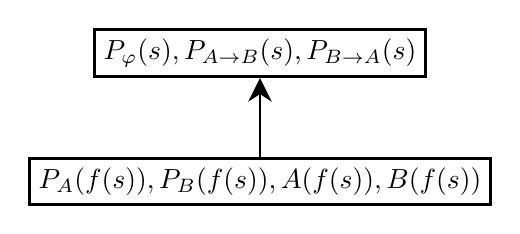
\begin{tikzpicture}[squarednode/.style={rectangle, draw, very thick, minimum size=5mm}]
				\node[squarednode]      (upper)                          {$P_\varphi(s), P_{A\to B}(s), P_{B\to A}(s)$};
				\node[squarednode]      (lower)       	[below=of upper] {$P_A(f(s)), P_B(f(s)), A(f(s)), B(f(s))$};
				\draw[-{Stealth[length=3mm, width=3mm]}] (lower.north) -- (upper.south);
			\end{tikzpicture}
		\end{center}
		
		i.e. for all $P, Q$ in the same rectangle have $P\precsim Q$ and $P\precsim Q$, and for $P$ in the lower $Q$ in the upper $P\prec Q$.
	\end{example}

	
	

	\chapter{Implementation}
		
	
	\bibliographystyle{plain}
	\bibliography{EIICL}
	
\end{document}